\documentclass{article}

\usepackage{listings}
\usepackage{pgfplots}

\begin{document}
\section{Optimal tile size for matrix multiplication}
The purpose of this test is to measure the performance characteristics of Biohadoop for a given problem. The problem is to find an optimal tile size for the tiled matrix multiplication.

A matrix multiplication can be performed in different ways. The most obvious one is the standard algorithm:
\begin{lstlisting}
for i = 1 to n
  for j = 1 to n
    for k = 1 to n
      C(i,j) = C(i,j) + A(i,k) * B(k,j)
\end{lstlisting}

The matrix multiplication can be improved by loop tiling (!!!cite!!!). The computation is performed on smaller blocks (tiles) of the matrices:
\begin{lstlisting}
for i0 = 1 to n, step blocksize_i
  for j0 = 1 to n, step blocksize_j
    for k0 = 1 to n, step blocksize_i
      for i = i0 to min(i0 + blocksize_i, n)
        for j = j0 to min(j0 + blocksize_j, n)
          for k = k0 to min(k0 + blocksize_i, n)
            C(i,j) = C(i,j) + A(i,k) * B(k,j)
\end{lstlisting}

If the blocks are small enough, they fit into the L1 CPU cache, which results in a speed up (!!!cite or show result!!!). Theoretically, the optimal block size (in terms of computation speed) can be computed by considering cache and block sizes (!!!example?!!!). But in a real environment, there are many other factors that influence the optimal tile size. One factor is the cache usage by the underlying OS. Another factor is the existence of L2 or L3 caches and their sizes. So we need to find an alternative way to get optimal tile sizes.

An optimization algorithm can be used to find the (near) optimal tile size. In this case, the optimization is done using a GA. Each individual in the population represents a tile size, where the tile size is defined by the values \texttt{blocksize\_i}, \texttt{blocksize\_j} and \texttt{blocksize\_k}. The fitness function is computed as the time it takes to multiply the matrices $A$ and $B$ using a given tile size. The goal is to find an optimal tile size, that minimizes the time to compute a matrix multiplication.

Each GA iteration computes the fitness values of the child population (!!!reference GA in chapter!!!). This fitness values, together with the values of the current population, are then used to determine the next iteration's GA population. Remember, to compute the fitness value for a given tile size, we have to do a matrix multiplication. So we have to compute $population\_size$ matrix multiplications in each iteration, and $iterations * population\_size$ matrix multiplications altogether.

%The GA is implemented with no optimizations (e.g. no reuse of already known results) and requires therefor lots of unnecessary computation repetitions, but the approach is good enough, as the real task is to find the scaling properties of Biohadoop for the given problem.

% Depending on the properties of the problem, the optimization can take a long time. The time determining properties are
% \begin{itemize}
%   \item Number of GA iterations
%   \item GA population size
%   \item Matrix size
% \end{itemize}

The computation of the fitness function takes the most time in the optimization (!!show data to support this statement!!). It can be parallelized easily, as different matrix multiplications don't depend on each other. So it is the perfect candidate for parallelization, which is done with Biohadoop.

On startup, each worker receives a full copy of the matrices $A$ and $B$ to minimize network transfers later on. Then, in each GA iteration, the GA distributes the tile sizes of the child population to the workers. The workers compute the matrix multiplication on $A$ and $B$ using the provided tile size. The time spent on this computation is returned to the GA, which considers it as the fitness value for the given tile size.

By distributing a full copy of matrices $A$ and $B$ in the initial phase, the network transmission is minimized during the work phase. In the work phase, only the tile size (Integer) is sent to a worker, which returns the time spent for the matrix multiplication (Long). This way, the network is not the bottleneck when trying to scale out (!!!add some numbers about network usage during work phase, to support this statement!!!).

Every worker runs in a distinct container, and so does the GA algorithm. For this tests, each container consist of 1 CPU and 128MB RAM. In the results shown below, the container for the GA algorithm is excluded, those containers are worker only containers.

\subsection{Algorithm parameters}
\label{algorithm-parameters}
\begin{itemize}
  \item Matrix size = 128x128
  \item Min tile size = 1
  \item Max tile size = 128
  \item GA population = 50
  \item GA iterations = 1000
  \item GA mutation factor = $\pm 32$
\end{itemize}

\subsection{Hardware}
\label{hardware}
Cluster of 6 machines, each machine has the following spec:
\begin{itemize}
  \item Intel Core2 Duo CPU E8200 @ 2.66GHz (2x2,66Ghz, no hyperthreading)
  \item 6MB shared L2 cache, 32KB L1 data cache, 32KB L1 instruction cache
  \item 4GB (2x2GB) DDR2 RAM @ 667MHz
\end{itemize}
All machines are connected through switched 1GB Ethernet network. The ping latency is about 0,12ms.

\subsection{Results}
(!!!! WHAT ABOUT WORKERS THAT RUN ON THE SAME MACHINE AS APPLICATIONMASTER?!!!!)
The tests were performed using the algorithm settings shown in section \ref{algorithm-parameters}. The hardware specification can be found in section \ref{hardware}. The tests differ in the number of used worker containers (and thus in the number of workers), that range from 1 to 18. To get more reliable results, each test was repeated 3 times.

\begin{figure}[h]
  \centering
  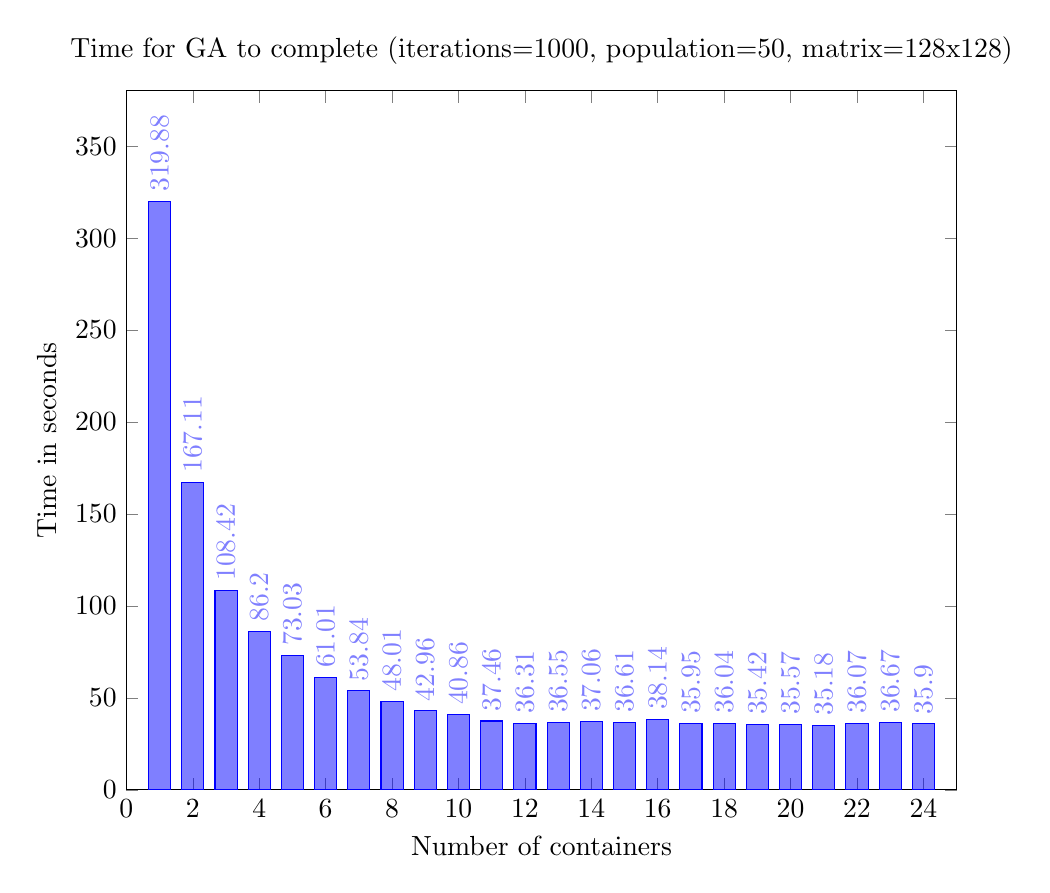
\begin{tikzpicture}[]
    \begin{axis}[
	title={Time for GA to complete (iterations=1000, population=50, matrix=128x128)},
	xlabel={Number of containers},
	ylabel={Time in seconds},
	width=\linewidth,
	enlargelimits=false,
	nodes near coords=\rotatebox{90}{\pgfmathprintnumber[]\value},
	visualization depends on=rawy \as \value,
	xmin=0,
	xmax=25,
	ymin=0,
	ymax=380
      ]
      \addplot[ybar, bar width=8pt, blue, fill, fill opacity=0.5]
      coordinates{(1,319.882333333) (2,167.111) (3,108.418333333) (4,86.2033333333) (5,73.0313333333) (6,61.0076666667) (7,53.838) (8,48.0086666667) (9,42.958) (10,40.855) (11,37.463) (12,36.313) (13,36.554) (14,37.059) (15,36.6086666667) (16,38.14) (17,35.9516666667) (18,36.0416666667) (19,35.4223333333) (20,35.5743333333) (21,35.1753333333) (22,36.065) (23,36.6666666667) (24,35.9003333333)};
%       \addplot [red, no markers] coordinates {(0,0) (12,38.4)};
    \end{axis}
  \end{tikzpicture}
  \caption{Find an optimal tile size for the tiled matrix multiplication. The x-axis shows the number of containers (workers), the y-axis shows the time it took to finish. iterations=1000, population=50, matrix size=128x128}
\label{plot:tiledmul1}
\end{figure}

\begin{figure}[h]
  \centering
  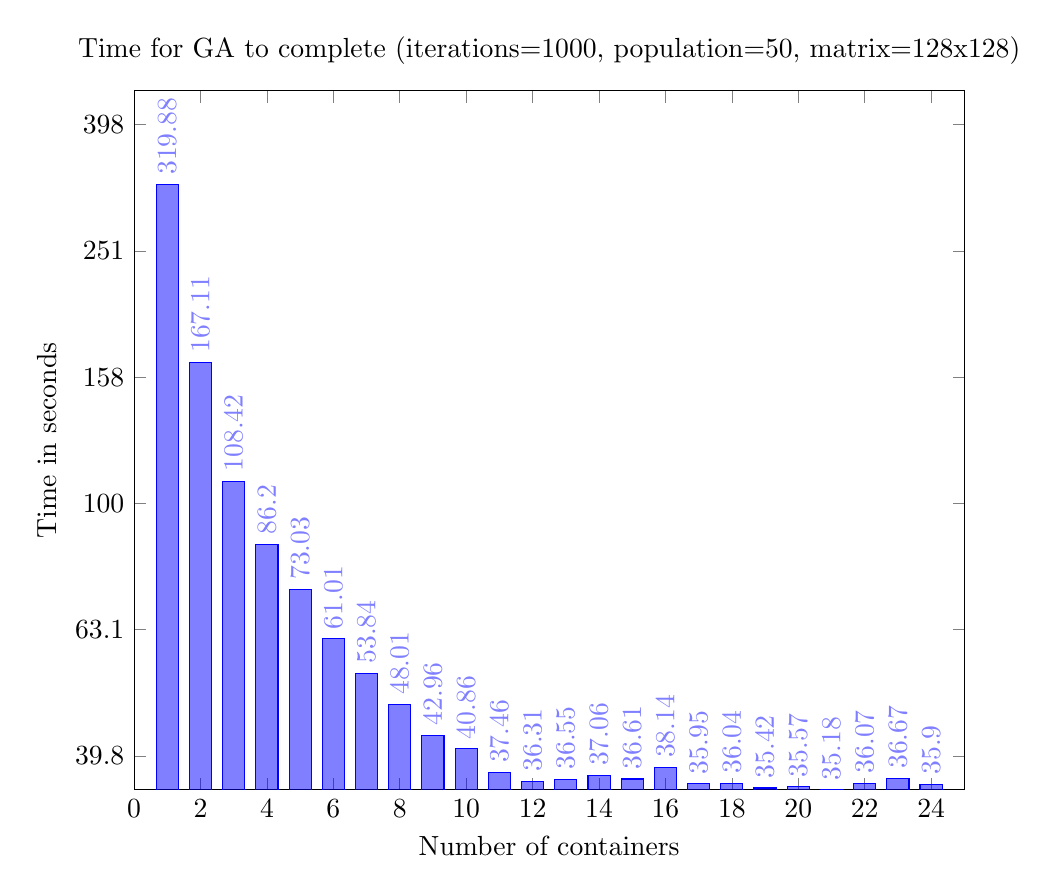
\begin{tikzpicture}[]
    \begin{semilogyaxis}[
	title={Time for GA to complete (iterations=1000, population=50, matrix=128x128)},
	xlabel={Number of containers},
	ylabel={Time in seconds},
	width=\linewidth,
	enlargelimits=false,
% 	nodes near coords,
	log ticks with fixed point,
	nodes near coords=\rotatebox{90}{\pgfmathprintnumber[]\value},
	visualization depends on=rawy \as \value,
	xmin=0,
	xmax=25,
	ymin=0,
	ymax=450
      ]
      \addplot[ybar, bar width=8pt, blue, fill, fill opacity=0.5]
      coordinates{(1,319.882333333) (2,167.111) (3,108.418333333) (4,86.2033333333) (5,73.0313333333) (6,61.0076666667) (7,53.838) (8,48.0086666667) (9,42.958) (10,40.855) (11,37.463) (12,36.313) (13,36.554) (14,37.059) (15,36.6086666667) (16,38.14) (17,35.9516666667) (18,36.0416666667) (19,35.4223333333) (20,35.5743333333) (21,35.1753333333) (22,36.065) (23,36.6666666667) (24,35.9003333333)};
    \end{semilogyaxis}
  \end{tikzpicture}
  \caption{Find an optimal tile size for the tiled matrix multiplication. The x-axis shows the number of containers (workers), the y-axis shows the time it took to finish on a logarithmic scale. iterations=1000, population=50, matrix size=128x128}
  \label{plot:tiledmul2}
\end{figure}

% ----128x128 with biohadoop-0.4.0-SNAPSHOT

\begin{figure}[h]
  \centering
  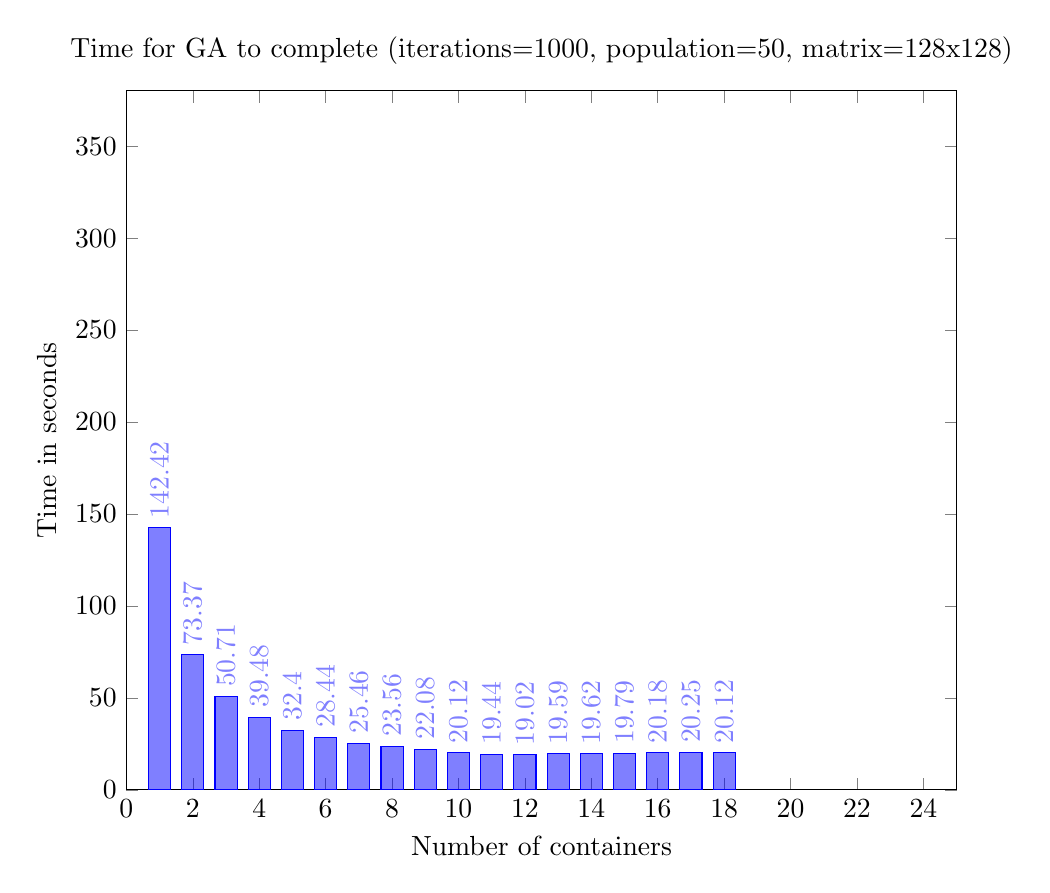
\begin{tikzpicture}[]
    \begin{axis}[
	title={Time for GA to complete (iterations=1000, population=50, matrix=128x128)},
	xlabel={Number of containers},
	ylabel={Time in seconds},
	width=\linewidth,
	enlargelimits=false,
	nodes near coords=\rotatebox{90}{\pgfmathprintnumber[]\value},
	visualization depends on=rawy \as \value,
	xmin=0,
	xmax=25,
	ymin=0,
	ymax=380
      ]
      \addplot[ybar, bar width=8pt, blue, fill, fill opacity=0.5]
      coordinates{(1,142.41692) (2,73.3701) (3,50.7134) (4,39.47686) (5,32.40048) (6,28.43836) (7,25.45766) (8,23.5593) (9,22.08228) (10,20.12404) (11,19.44024) (12,19.02386) (13,19.59172) (14,19.61892) (15,19.79174) (16,20.17862) (17,20.25264) (18,20.12062)};
%       \addplot [red, no markers] coordinates {(0,0) (12,38.4)};
    \end{axis}
  \end{tikzpicture}
  \caption{Find an optimal tile size for the tiled matrix multiplication. The x-axis shows the number of containers (workers), the y-axis shows the time it took to finish. iterations=1000, population=50, matrix size=128x128}
\label{plot:tiledmul5}
\end{figure}

\begin{figure}[h]
  \centering
  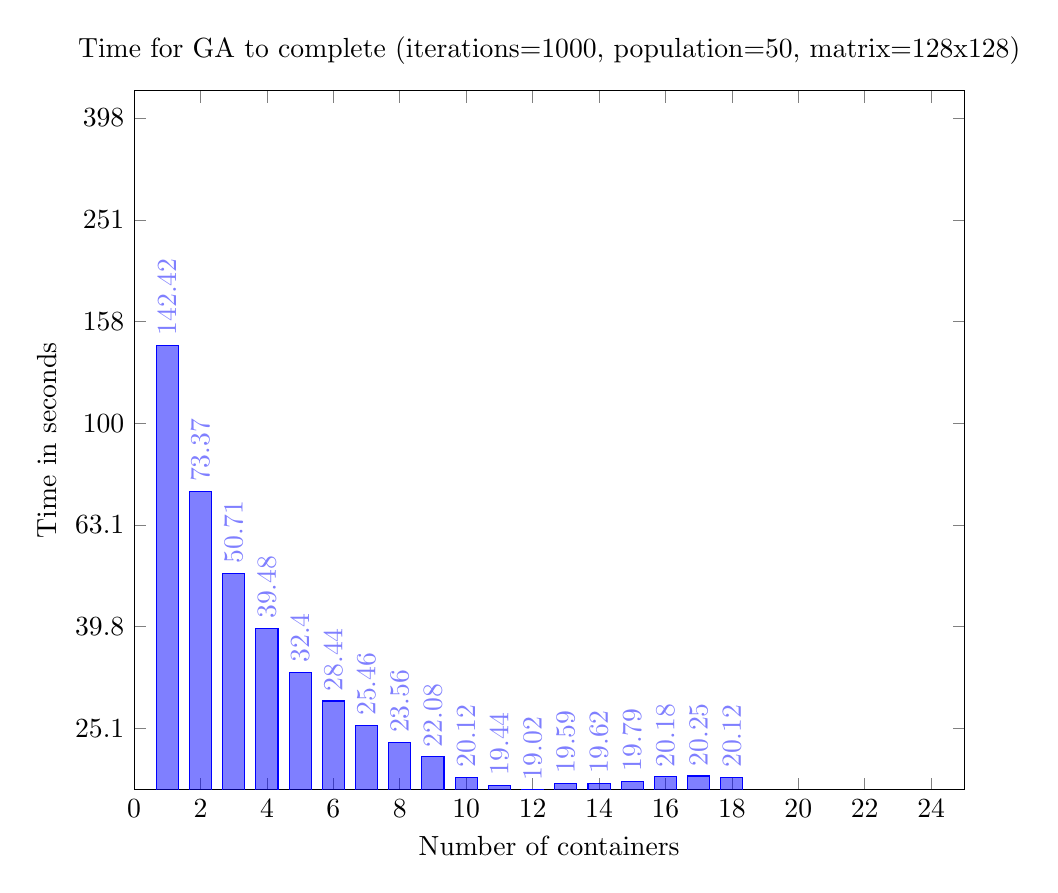
\begin{tikzpicture}[]
    \begin{semilogyaxis}[
	title={Time for GA to complete (iterations=1000, population=50, matrix=128x128)},
	xlabel={Number of containers},
	ylabel={Time in seconds},
	width=\linewidth,
	enlargelimits=false,
% 	nodes near coords,
	log ticks with fixed point,
	nodes near coords=\rotatebox{90}{\pgfmathprintnumber[]\value},
	visualization depends on=rawy \as \value,
	xmin=0,
	xmax=25,
	ymin=0,
	ymax=450
      ]
      \addplot[ybar, bar width=8pt, blue, fill, fill opacity=0.5]
      coordinates{(1,142.41692) (2,73.3701) (3,50.7134) (4,39.47686) (5,32.40048) (6,28.43836) (7,25.45766) (8,23.5593) (9,22.08228) (10,20.12404) (11,19.44024) (12,19.02386) (13,19.59172) (14,19.61892) (15,19.79174) (16,20.17862) (17,20.25264) (18,20.12062)};
    \end{semilogyaxis}
  \end{tikzpicture}
  \caption{Find an optimal tile size for the tiled matrix multiplication. The x-axis shows the number of containers (workers), the y-axis shows the time it took to finish on a logarithmic scale. iterations=1000, population=50, matrix size=128x128}
  \label{plot:tiledmul6}
\end{figure}

% ----256x256

\begin{figure}[h]
  \centering
  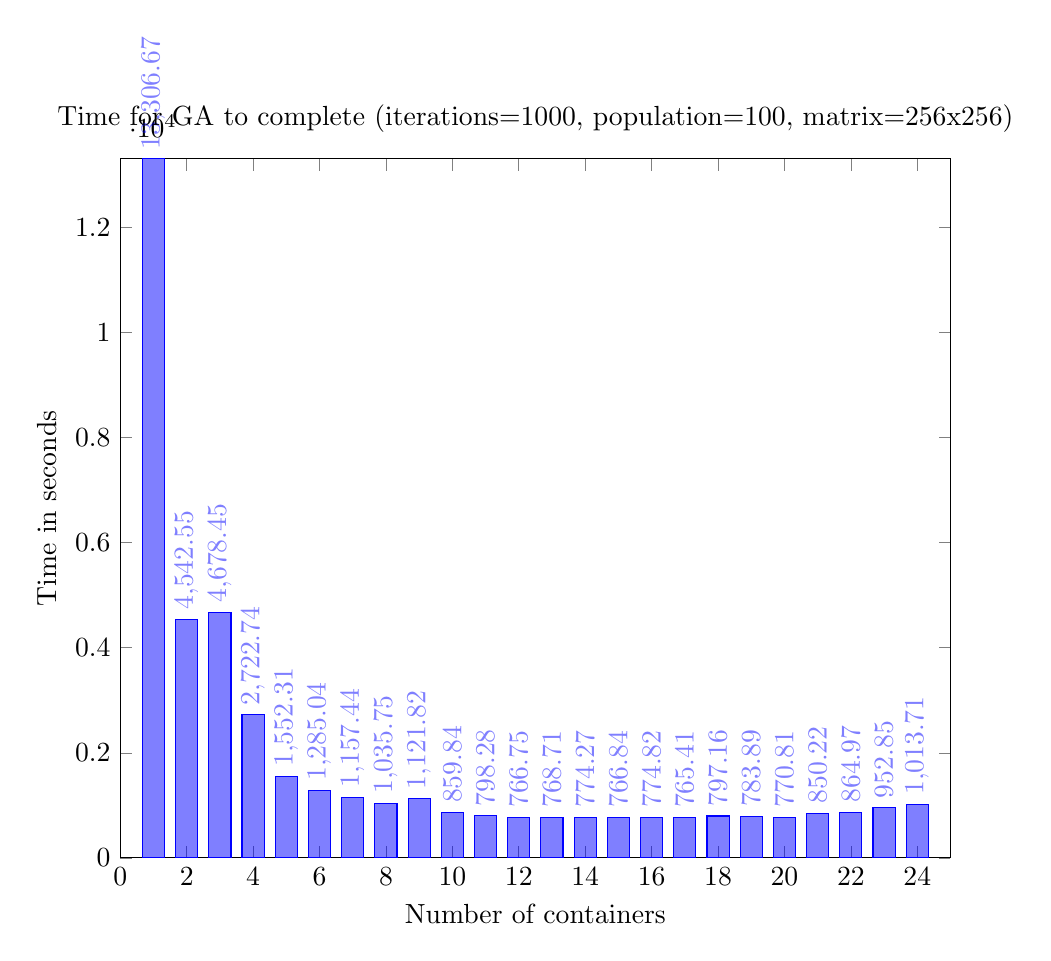
\begin{tikzpicture}[]
    \begin{axis}[
	title={Time for GA to complete (iterations=1000, population=100, matrix=256x256)},
	xlabel={Number of containers},
	ylabel={Time in seconds},
	width=\linewidth,
	enlargelimits=false,
	nodes near coords=\rotatebox{90}{\pgfmathprintnumber[]\value},
	visualization depends on=rawy \as \value,
	xmin=0,
	xmax=25,
	ymin=0
% 	ymax=380
      ]
      \addplot[ybar, bar width=8pt, blue, fill, fill opacity=0.5]
      coordinates{(1,13306.67) (2,4542.554) (3,4678.45266667) (4,2722.74433333) (5,1552.311) (6,1285.038) (7,1157.44166667) (8,1035.745) (9,1121.818) (10,859.836) (11,798.275666667) (12,766.746) (13,768.711333333) (14,774.27) (15,766.840333333) (16,774.817333333) (17,765.406) (18,797.155) (19,783.889333333) (20,770.809333333) (21,850.216666667) (22,864.974333333) (23,952.846) (24,1013.713)};
%       \addplot [red, no markers] coordinates {(0,0) (12,38.4)};
    \end{axis}
  \end{tikzpicture}
  \caption{Find an optimal tile size for the tiled matrix multiplication. The x-axis shows the number of containers (workers), the y-axis shows the time it took to finish. iterations=1000, population=100, matrix size=256x256}
\label{plot:tiledmul3}
\end{figure}

\begin{figure}[h]
  \centering
  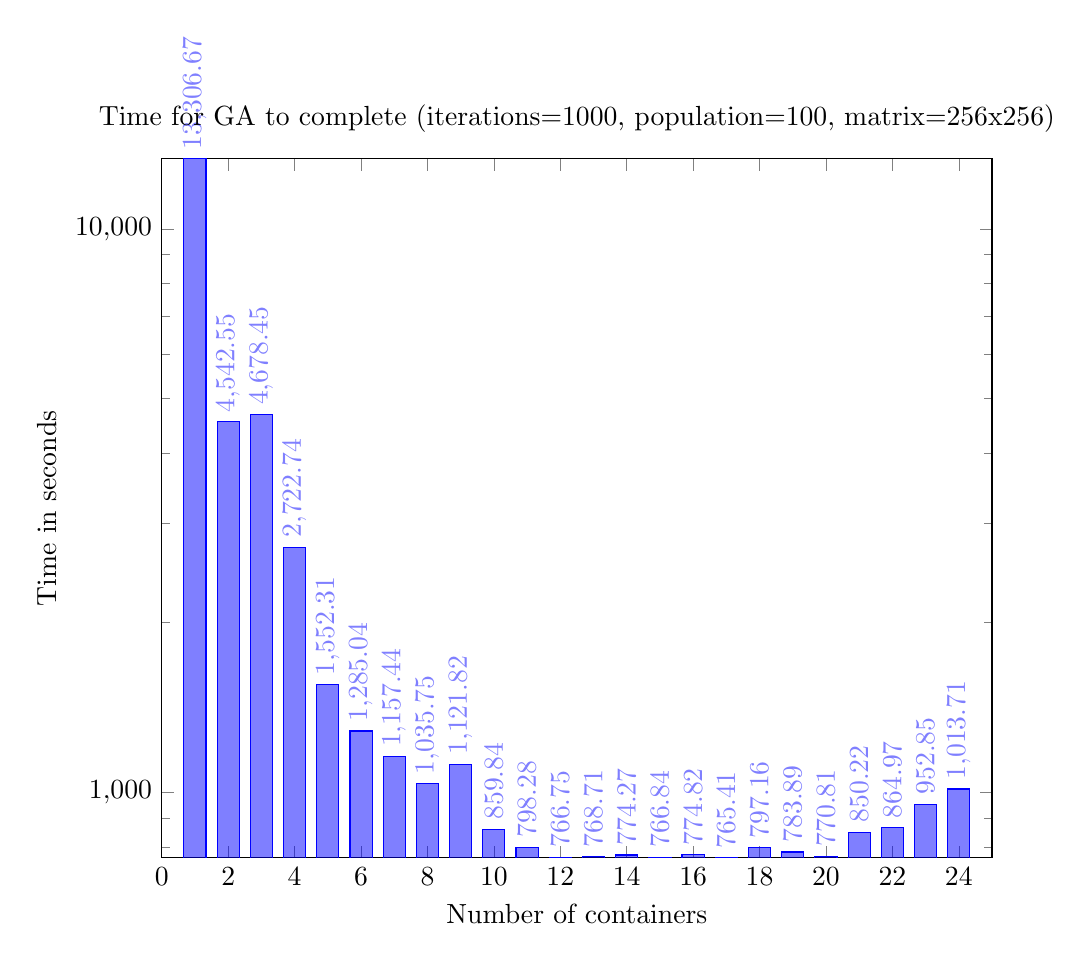
\begin{tikzpicture}[]
    \begin{semilogyaxis}[
	title={Time for GA to complete (iterations=1000, population=100, matrix=256x256)},
	xlabel={Number of containers},
	ylabel={Time in seconds},
	width=\linewidth,
	enlargelimits=false,
% 	nodes near coords,
	log ticks with fixed point,
	nodes near coords=\rotatebox{90}{\pgfmathprintnumber[]\value},
	visualization depends on=rawy \as \value,
	xmin=0,
	xmax=25,
	ymin=0
% 	ymax=450
      ]
      \addplot[ybar, bar width=8pt, blue, fill, fill opacity=0.5]
      coordinates{(1,13306.67) (2,4542.554) (3,4678.45266667) (4,2722.74433333) (5,1552.311) (6,1285.038) (7,1157.44166667) (8,1035.745) (9,1121.818) (10,859.836) (11,798.275666667) (12,766.746) (13,768.711333333) (14,774.27) (15,766.840333333) (16,774.817333333) (17,765.406) (18,797.155) (19,783.889333333) (20,770.809333333) (21,850.216666667) (22,864.974333333) (23,952.846) (24,1013.713)};
    \end{semilogyaxis}
  \end{tikzpicture}
  \caption{Find an optimal tile size for the tiled matrix multiplication. The x-axis shows the number of containers (workers), the y-axis shows the time it took to finish on a logarithmic scale. iterations=1000, population=100, matrix size=256x256}
  \label{plot:tiledmul4}
\end{figure}

As we can see from figure \ref{plot:tiledmul1} and \ref{plot:tiledmul2}, the problem scales up to 12 containers. After that, the performance remains the same, with small fluctuations in both directions (!!!explain reasons for fluctuations: matrix multiplication takes different time for different tile sizes, if during GA iterations bad tiles sizes are chosen, iteration takes longer. other reasons: CPU cache, multiprocess OS, network)!!!). This seems plausible, as the whole cluster provides 12 physical cores. Each container allocates one core, and each matrix multiplication consumes almost 100\% of a given core (!!! add data !!!). After the 12 cores are fully occupied, each new container has to compete for resources with the other containers, that run on the same machine - the cluster is fully occupied. Figure \ref{plot:tiledmul2} shows the results 1in logarithmic form - the data is the same as in figure \ref{plot:tiledmul1}.

(!!! compare scale of this test problem with other implementations? !!!)

Reasons for the speed up degradation in the interval from 1 to 12 are (!!!need to prove with data!!!):
\begin{itemize}
  \item The GA itself needs some time to run. This part of the algorithm runs sequentially (!!!Amdahls Law!!!). The size of the sequential part depends on the GA population size and the matrix size (!!!measure with different population/matrix sizes and compare!!!)
  \item The GA itself runs on one of the cluster machines, consuming resources (!!!Idea: run Biohadoop on single node and force workers to run on other nodes (use rack affinity); Compare results with this result!!!)
  \item The communication between the machines takes some time (netty pipeline, OS, network) (!!!to get data, measure echo speed with same messages as matrix mul, but no algorithm overhead!!!)
\end{itemize}

\subsection{TODO}
\begin{itemize}
  \item Find time for sequential part (GA) and parallel part (matrix mul + network). Compute max. speedup. Discuss results and compare with test data
  \item Discuss speed degradation issues in further detail
  \item replace figure \ref{plot:tiledmul2} with a table, showing the speeups?
  \item ???
\end{itemize}


\end{document}
